\newpage
\datos{color}{}{}
\section{[2 puntos] Ejercicio 2}
%\addcontentsline{toc}{section}{Ejercicio 1}
\textbf{Considera un programa en CLIPS que permita hacer menús dietéticos.
Para ello por una parte se indicarán ingredientes, por ejemplo:}

\begin{center}
    \textbf{(fruta manzana calorias 40)}\\
    \textbf{(carne ternera calorias 220)}\\
\end{center}

\textbf{A partir de estos, escribir reglas para crear los menús:}
\begin{enumerate}[label=\alph*)]
    \item \textbf{Un menú se compone de primer plato, segundo plato y postre}.
    \item \textbf{El postre tiene que ser fruta, pastel o café}.
    \item \textbf{De segundo puede haber carne, pescado u opción vegana}. \\
\end{enumerate}

\textbf{El programa debería permitir crear menús a partir de los ingredientes que
cumplieran alguna restricción calórica. En caso de que no haya solución, habrá que
sacar un mensaje diciendo “No comas”.} \\

Con el fin de mantener coherencia con el ámbito sobre el que se basa el ejemplo, el sistema
diseñado no puede repetir tipo de plato en un mismo menú, es decir, si el primer plato 
es pescado, el segundo solo podrá ser carne u opción vegana. \\

Además, el sistema solo puede tener una única restricción calórica en activo. No obstante,
después de generar menús con una restricción calórica, en caso de modificarla y generar 
nuevos con otra restricción calórica, se mantienen los menús anteriores en el sistema,
esto es, no se eliminan. \\

El sistema diseñado e implementado dispone de un menú interactivo por terminal 
que provee de las siguiente funciones:
\begin{multicols}{2}
\begin{itemize}
    \item 0. Inicializar sistema (reset)
    \item 1. Añadir ingrediente
    \item 2. Eliminar ingrediente
    \item 3. Ver ingredientes
    \item 4. Establecer restricción calórica
    \item 5. Ver restricción calórica actual
    \item 6. Generar menús
    \item 7. Ver menús generados
    \item 8. Guardar hechos en fichero
    \item 9. Cargar hechos desde fichero
    \item 10. Salir
\end{itemize}
\end{multicols}

\subsection{Ejecución del sistema}
Con CLIPS instalado en el equipo, abrir una terminal \textit{bash} y proceder como se
describe a continuación:
\begin{lstlisting}[style=clipsstyle, caption={Ejecución del sistema del ejercicio 2 en CLIPS.}, label={lst:menu-ejemplo}]
clips
(load "ejercicio2.clp") # si el fichero se encuentra en la ruta actual
(menu)
\end{lstlisting}

\vspace{0.2cm}
Este procedimiento se muestra en la Figura \ref{fig:ejecutarClips}.
\begin{figure}[h!]
    \centering
    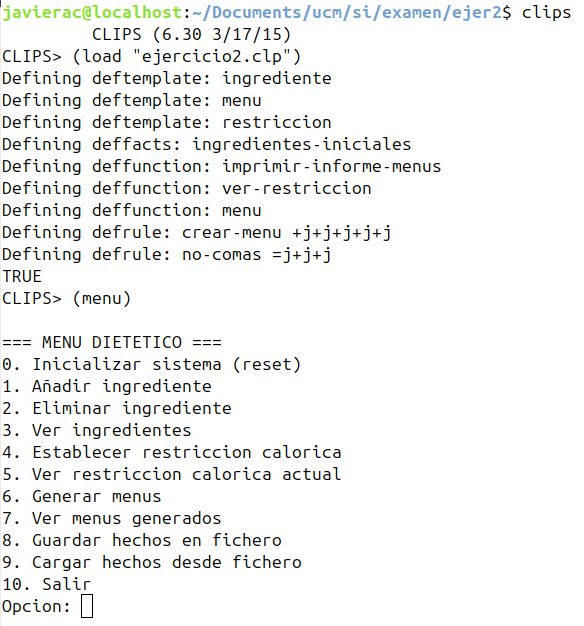
\includegraphics[width=0.7\textwidth]{Images/ejer2/ejecutarClips.png}
    \caption{Ejecución del sistema del ejercicio 2 en CLIPS.}
    \label{fig:ejecutarClips}
\end{figure}


\clearpage
\subsection{Plan de pruebas del sistema diseñado e implementado}
Con el objetivo de validar el correcto funcionamiento del sistema desarrollado y su 
adecuación a los requisitos del enunciado se han probado los casos descritos en la 
Tabla \ref{tab:pruebasClips}. Estos casos se han realizado utilizando las opciones
del menú interactivo.

\begin{table}[h!]
\centering

% --- CABECERA ---
\begin{tabular}{|
    >{\columncolor{black}\color{white}}p{0.4cm} |
    >{\columncolor{black}\color{white}}p{4cm} |
    >{\columncolor{black}\color{white}}p{10cm} |
}
\hline
\textbf{} & \textbf{Caso} & \textbf{Resultado esperado} \\
\hline
\end{tabular}

% --- CUERPO ---
\begin{tabular}{|
    >{\columncolor{black}\color{white}}c |
    p{4cm} |
    p{10cm} |
}
\hline
1 & Inicialización & Se cargan los ingredientes iniciales del sistema. \\
\hline
2 & Ver ingredientes & Se muestran todos los ingredientes disponibles. \\
\hline
3 & Establecer restricción & Se crea la restricción calórica. \\
\hline
4 & Ver restricción & Se muestra la restricción actual correcta. \\
\hline
5 & Generar menús válidos & Se generan menús que cumplen todas las reglas del sistema. \\
\hline
6 & Ver menús & Se listan los menús generados. \\
\hline
7 & Restricción demasiado baja & No se genera ningún menú y se muestra “No comas". \\
\hline
8 & Añadir ingrediente & Se añade correctamente un nuevo ingrediente. \\
\hline
9 & Generar menús tras añadir & Se generan menús válidos con el nuevo ingrediente. \\
\hline
10 & Eliminar ingrediente & Se elimina el ingrediente seleccionado. \\
\hline
11 & Guardar hechos & Se guarda un archivo con los hechos actuales. \\
\hline
12 & Cargar hechos & Se cargan los hechos desde un archivo. \\
\hline
13 & Doble restricción & Solo queda activa la última restricción establecida. \\
\hline
14 & Ver restricción tras cambio & Se muestra la nueva restricción. \\
\hline
15 & Sin restricción válida (no se ha establecido) & No se genera ningún menú y se muestra “No comas”. \\
\hline
\end{tabular}

\caption{Casos de prueba del sistema del ejercicio 2 en CLIPS.}
\label{tab:pruebasClips}
\end{table}

\subsection{Código de la implementación del sistema en CLIPS}
Se ha reutilizado la resolución propuesta al ejercicio del segundo tema realizado 
a lo largo de la asignatura. La implementación del ejercicio actual se presenta en 
el Código \ref{cod:clips-sistema}.

\lstinputlisting[
    style=clipsstyle2,
    caption={Implementación del sistema del ejercicio 2 en CLIPS},
    label={cod:clips-sistema}
]{Code/ejercicio2.clp}

\subsection{Resultados}
En las Figuras \ref{fig:rdoClips} y \ref{fig:rdoClips2} se muestra el resultado de la ejecución del sistema.
Concretamente, se observa su capacidad para generar menús cumpliendo tanto la restricción
calórica como las restricciones de tipos de ingredientes en cada plato.

\begin{figure}[h!]
    \centering
    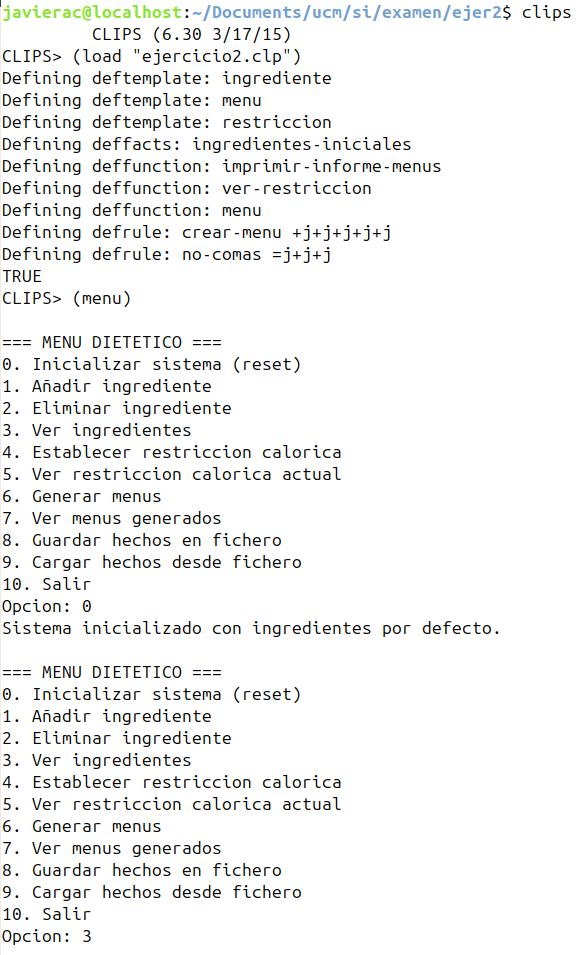
\includegraphics[scale=0.35]{Images/ejer2/rdo1.png}
    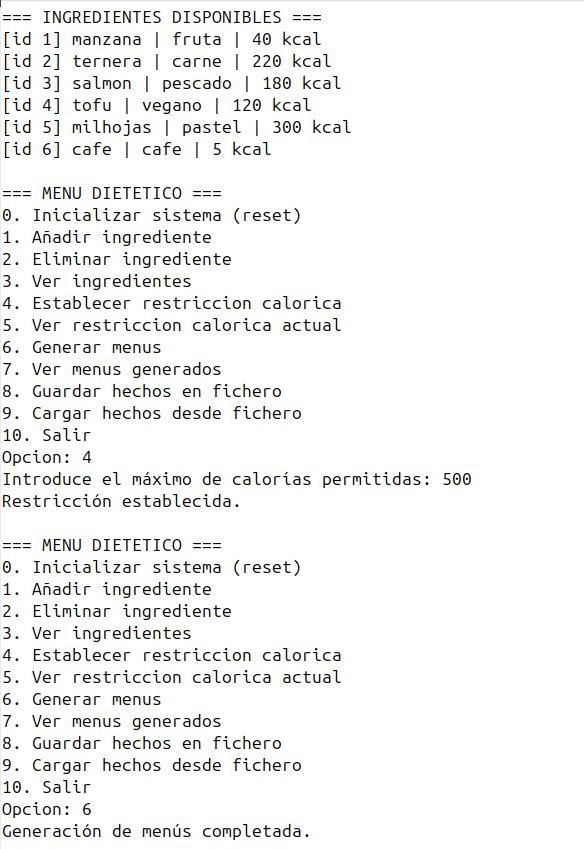
\includegraphics[scale=0.35]{Images/ejer2/rdo2.png}
    \caption{Resultado de la ejecución del sistema del ejercicio 2 en CLIPS.}
    \label{fig:rdoClips}
\end{figure}

\begin{figure}[h!]
    \centering
    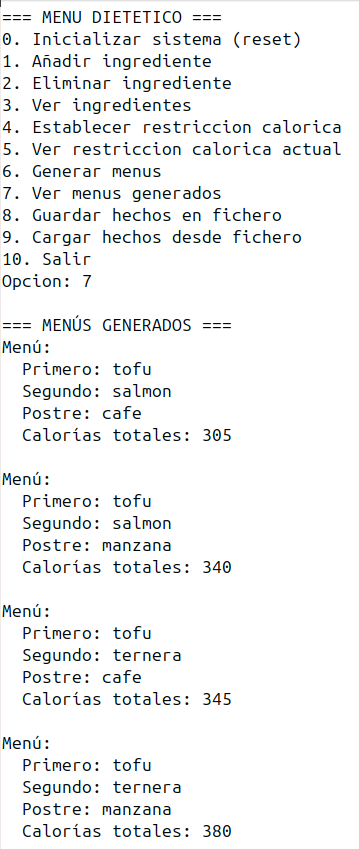
\includegraphics[scale=0.45]{Images/ejer2/rdo3.png}
    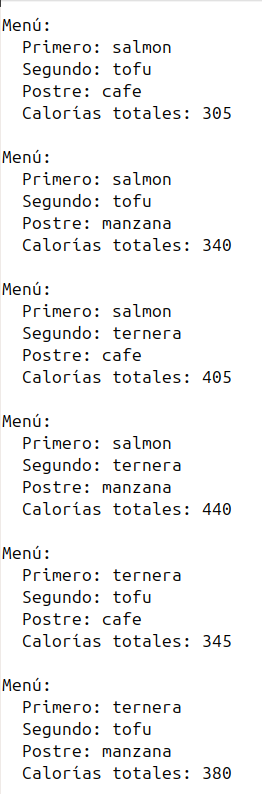
\includegraphics[scale=0.45]{Images/ejer2/rdo4.png}
    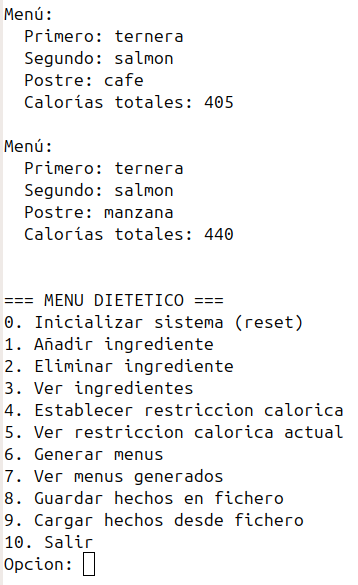
\includegraphics[scale=0.45]{Images/ejer2/rdo5.png}
    \caption{(continuación) Resultado de la ejecución del sistema del ejercicio 2 en CLIPS.}
    \label{fig:rdoClips2}
\end{figure}